\documentclass[a4paper, 10pt, ]{article}

\usepackage[slovak]{babel}





\usepackage[utf8]{inputenc}
\usepackage[T1]{fontenc}

\usepackage[left=4cm,
			right=4cm,
            % left=2.5cm,
			% right=5.5cm,
			top=2.1cm,
			bottom=2.6cm,
			footskip=7.5mm,
			% twoside,
			marginparwidth=3.0cm,
			%showframe,
			]{geometry}

\usepackage{graphicx}
\usepackage[dvipsnames]{xcolor}
% https://en.wikibooks.org/wiki/LaTeX/Colors


% ------------------------------

\usepackage{lmodern}

\usepackage[tt={oldstyle=false,proportional=true,monowidth}]{cfr-lm}

% ------------------------------

\usepackage{amsmath}
\usepackage{amssymb}
\usepackage{amsthm}

\usepackage{booktabs}
\usepackage{multirow}
\usepackage{array}
\usepackage{dcolumn}


\usepackage[singlelinecheck=true]{subfig}


% ------------------------------


\def\naT{\mathsf{T}}

\hyphenpenalty=6000
\tolerance=1000




% ------------------------------


\makeatletter

	\def\@seccntformat#1{\protect\makebox[0pt][r]{\csname the#1\endcsname\hspace{4mm}}}

	\def\cleardoublepage{\clearpage\if@twoside \ifodd\c@page\else
	\hbox{}
	\vspace*{\fill}
	\begin{center}
	\phantom{}
	\end{center}
	\vspace{\fill}
	\thispagestyle{empty}
	\newpage
	\if@twocolumn\hbox{}\newpage\fi\fi\fi}

	\newcommand\figcaption{\def\@captype{figure}\caption}
	\newcommand\tabcaption{\def\@captype{table}\caption}

\makeatother


% ------------------------------




\usepackage{fancyhdr}
\fancypagestyle{plain}{%
\fancyhf{} % clear all header and footer fields
\fancyfoot[C]{\sffamily {\bfseries \thepage}\ | {\scriptsize\oznacenieCasti}}
\renewcommand{\headrulewidth}{0pt}
\renewcommand{\footrulewidth}{0pt}}
\pagestyle{plain}


% ------------------------------


\usepackage{titlesec}
\titleformat{\paragraph}[hang]{\sffamily  \bfseries}{}{0pt}{}
\titlespacing*{\paragraph}{0mm}{3mm}{1mm}
\titlespacing*{\subparagraph}{0mm}{3mm}{1mm}

\titleformat*{\section}{\sffamily\Large\bfseries}
\titleformat*{\subsection}{\sffamily\large\bfseries}
\titleformat*{\subsubsection}{\sffamily\normalsize\bfseries}






% ------------------------------

\PassOptionsToPackage{hyphens}{url}
\usepackage[pdfauthor={},
			pdftitle={},
			pdfsubject={},
			pdfkeywords={},
			% hidelinks,
			colorlinks=false,
			breaklinks,
			]{hyperref}


% ------------------------------


\graphicspath{%
{../fig_standalone/}%
{../../PY/fig/}%
{../../PY/jupynotex/fig/}%
{../../ML/fig/}%
{./fig/}%
}



% ------------------------------

\usepackage{enumitem}

\usepackage{lettrine}

% ------------------------------


\usepackage{microtype}


% ------------------------------

\usepackage[titles]{tocloft}

\setlength{\cftsecindent}{-12mm}
\setlength{\cftsecnumwidth}{12mm}
\renewcommand{\cftsecpresnum}{\hfill}
\renewcommand{\cftsecaftersnum}{\hspace{4mm}}

\setlength{\cftsubsecindent}{-12mm}
\setlength{\cftsubsecnumwidth}{16mm} % 12 + 4
\renewcommand{\cftsubsecpresnum}{\hfill}
\renewcommand{\cftsubsecaftersnum}{\hspace{8mm}} % 4 + 4 mm

\setlength{\cftsubsubsecindent}{-12mm}
\setlength{\cftsubsubsecnumwidth}{20mm} % 12 + 4 + 4
\renewcommand{\cftsubsubsecpresnum}{\hfill}
\renewcommand{\cftsubsubsecaftersnum}{\hspace{12mm}} % 4 + 4 + 4 mm

\renewcommand{\cftsecpagefont}{\lstyle \bfseries}
\renewcommand{\cftsubsecpagefont}{\lstyle}
\renewcommand{\cftsubsubsecpagefont}{\lstyle}



\setlength{\cftparaindent}{-16mm}
\setlength{\cftparanumwidth}{28mm} % 16 + 4 + 4 + 4
\renewcommand{\cftparapresnum}{\hfill}
\renewcommand{\cftparaaftersnum}{\hspace{16mm}} % 4 + 4 + 4 + 4 mm








% ------------------------------

\usepackage{listings}



\renewcommand{\lstlistingname}{Výpis kódu}
\renewcommand{\lstlistlistingname}{Výpisy kódu}




%New colors defined below
\definecolor{codegreen}{rgb}{0,0.6,0}
\definecolor{codegray}{rgb}{0.5,0.5,0.5}
\definecolor{codepurple}{rgb}{0.58,0,0.82}
\definecolor{backcolour}{rgb}{0.95,0.95,0.95}

%Code listing style named "mystyle"
\lstdefinestyle{mystyle}{
  backgroundcolor=\color{backcolour},
  commentstyle=\fontfamily{lmtt}\fontsize{8.5pt}{8.75pt}\selectfont\color{codegreen},
  keywordstyle=\fontfamily{lmtt}\fontsize{8.5pt}{8.75pt}\selectfont\bfseries\color{Blue},
  stringstyle=\fontfamily{lmtt}\fontsize{8.5pt}{8.75pt}\selectfont\color{codepurple},
  basicstyle=\fontfamily{lmtt}\fontsize{8.5pt}{8.75pt}\selectfont,
  breakatwhitespace=false,
  breaklines=true,
  captionpos=t,
  keepspaces=true,
  numbers=left,
  numbersep=4mm,
  numberstyle=\fontfamily{lmtt}\fontsize{8.5pt}{8.75pt}\selectfont\color{lightgray},
  showspaces=false,
  showstringspaces=false,
  showtabs=false,
  tabsize=2,
  % xleftmargin=10pt,
  framesep=10pt,
  language=Python,
  escapechar=|,
}


\lstset{
    inputencoding=utf8,
    extendedchars=true,
    literate=%
    {á}{{\'a}}1
    {č}{{\v{c}}}1
    {ď}{{\v{d}}}1
    {é}{{\'e}}1
    {ě}{{\v{e}}}1
    {í}{{\'i}}1
    {ň}{{\v{n}}}1
    {ó}{{\'o}}1
    {ř}{{\v{r}}}1
    {š}{{\v{s}}}1
    {ť}{{\v{t}}}1
    {ú}{{\'u}}1
    {ů}{{\r{u}}}1
    {ý}{{\'y}}1
    {ž}{{\v{z}}}1
    {Á}{{\'A}}1
    {Č}{{\v{C}}}1
    {Ď}{{\v{D}}}1
    {É}{{\'E}}1
    {Ě}{{\v{E}}}1
    {Í}{{\'I}}1
    {Ň}{{\v{N}}}1
    {Ó}{{\'O}}1
    {Ř}{{\v{R}}}1
    {Š}{{\v{S}}}1
    {Ť}{{\v{T}}}1
    {Ú}{{\'U}}1
    {Ů}{{\r{U}}}1
    {Ý}{{\'Y}}1
    {Ž}{{\v{Z}}}1
    {ô}{{\^{o}}}1
}


% ------------------------------


\usepackage{caption}

\DeclareCaptionFormat{odsadene}{\protect\makebox[0pt][r]{#1#2\hspace{4mm}}#3\par}
\DeclareCaptionLabelSeparator{lendvojbodka}{:}
% \DeclareCaptionFont{lightgray}{\color{lightgray}}
\DeclareCaptionFont{lightgray}{\fontfamily{lmtt}\fontsize{8.5pt}{8.75pt}\selectfont\color{lightgray}}

\captionsetup[lstlisting]{format=odsadene, labelsep=lendvojbodka, justification=raggedright, singlelinecheck=false, labelfont={sf, lightgray},}


% ------------------------------





% ------------------------------

\usepackage[backend=biber,
            style=numeric,
            sorting=none,
            ]{biblatex}
\DeclareSourcemap{
    \maps[datatype=bibtex]{
        \map{
        \step[fieldset=note, null]
        }
        \map{
        \step[fieldset=file, null]
        }        
        % \map{
        % \step[fieldset=url, null]        
        % }
        \map{
        \step[fieldset=eprint, null]
        }
    }
}


\addbibresource{E:/_CurrentContent/01_work_repo/bibLaTeXDB/bibLaTeXDB.bib} % nonpublic data





\def\oznacenieCasti{MRS01 - ZS2023}



\usepackage{pdflscape}
\usepackage{longtable}



\begin{document}


\lstset{%
style=mystyle,
rangebeginprefix=\#\#\#\ cellB\ ,%
rangebeginsuffix=\ \#\#\#,%
rangeendprefix=\#\#\#\ cellE\ ,%
rangeendsuffix=\ \#\#\#,%
includerangemarker=false,
}





\fontsize{12pt}{22pt}\selectfont

\centerline{\textsf{Modelovanie a riadenie systémov} \hfill \textsf{\oznacenieCasti}}

\fontsize{18pt}{22pt}\selectfont





\begin{flushleft}
	\textbf{\textsf{Úvod}}
\end{flushleft}






\normalsize

\bigskip

{\hypersetup{hidelinks}

\tableofcontents

}

\bigskip

\vspace{18pt}



\noindent
\lettrine[lines=3, nindent=0pt]{C}{ieľom} tohto textu je najmä vytvoriť akýsi úvodný zoznam pojmov, s ktorými potrebuje čitateľ pracovať pri štúdiu v oblasti kybernetiky, robotiky, teórie riadenia a tak podobne. Vo všeobecnosti ide o~značne široké pojmy avšak v~tomto texte je možné vidieť ako sa s nimi pracuje z hľadiska technickej kybernetiky, z~hľadiska (technickej) teórie systémov, z~hľadiska automatizácie a~z~hľadiska riadiacich systémov.








\section{Myšlienky na úvod}

Predmet \emph{Modelovanie a riadenie systémov} možno rozdeliť na dve hlavné časti: modelovanie systémov a riadenie systémov. Pre obe časti platí, že ide o prvotný súbor informácii pre čitateľa, ktorého cieľom je štúdium kybernetiky, robotiky, prípadne ďalej teórie riadenia, identifikácie systémov atď. (veľmi rozsiahle možnosti).

Pre prácu v tomto predmete (alebo v týchto oblastiach) je prakticky nevyhnutné využívať isté nástroje, tu sa tým myslia znalosti a praktické zručnosti najmä (ale nie len) z matematiky - diferenciálny a integrálny počet, práca s maticami a algebra. Predmet nie je zameraný na tieto oblasti. Predmet ich využíva. Je veľmi výhodné ak sa študent s~využívaním týchto nástrojov stretol v minulosti, ale nie je to nevyhnutné. Všetko potrebné bude obsiahnuté v predmete, avšak často len v minimálnej miere s~tým, že čitateľ by mal mať jasno v tom akým smerom vo využívaní týchto nástrojov (matematiky napríklad) by sa mal vydať.

Veľmi súvisiacou sadov nástrojov, ktoré je tu potrebné využívať, je výpočtový softvér, typu MATLAB, GNU Octave, knižnice NumPy pre Python a podobné knižnice pre iné skriptovacie jazyky ako Julia, R a podobne. Rovnako však platí, že v rámci predmetu bude poskytnuté všetko potrebné pre úspešnú prácu a pre ďalšie rozširovanie si vedomostí, skúseností a zručností (v jednom predmete samozrejme nie je možné obsiahnuť všetko).

Hlavným cieľom predmetu je teda vytvoriť priestor pre prvý kontakt s pojmami diskutovanými nižšie avšak nie vo všeobecnosti ale z hľadiska kybernetiky, teórie riadenia, automatizácie a tak podobne.





\subsection{Kybernetika}

\begin{itemize}[leftmargin=0pt, labelsep=3mm, itemsep=0pt]
    \item Veda o riadení a komunikácii v dynamických systémoch.
    \item Skúma spoločné zákonitosti na základe analógie medzi systémami rôznej fyzickej podstaty (fyzika - mechanika - elektrotechnika)
    \item Kybernetika - veda o:
    \begin{itemize}
        \item modelovaní a riadení procesov
        \item získavaní informácií a riadení
        \item riadení a komunikácii v dynamických systémoch
    \end{itemize}
    \item Metódami kybernetiky sú systémový prístup a modelovanie pri riešení problémov.
\end{itemize}



\subsection{Spätná väzba v systéme}

Spätná väzba predstavuje prenos a spätný návrat informácie. Vyskytuje sa bežne v~prírode.

Spätná väzba môže byť:
\begin{itemize}
    \item Záporná (negatívna) alebo
    \item Kladná (pozitívna)
\end{itemize}

Kladná spätná väzba vychyľuje systém smerom preč od rovnováhy.


\paragraph{Kladná spätná väzba (príklady)}

Je potrebné zobrať dva mobilné telefóny. Zavolať z jedného na druhý a po nadviazaní spojenia ich dať oba do hlasného režimu. Potom ich priblížiť displejmi k sebe, na vzdialenosť tak 10 cm. A nakoniec niečo povedať alebo zapískať. Z reproduktorov mobilov sa ozve nepríjemný, výrazný zvuk, ktorý sa podarí prerušiť len oddialením oboch telefónov.

To čo sa Vám podarilo vytvoriť, je akustická \emph{kladná spätná väzba}. Tento jav funguje na princípe neustáleho cyklického zosilňovania zvuku. Najprv jeden z telefónov svojim mikrofónom zachytí aj úplne nepatrný zvuk a pošle ho cez mobilnú sieť druhému telefónu. Ten prijatý zvuk prehrá na svojom reproduktore. Takto zosilnený zvuk opäť zachytí prvý telefón svojim mikrofónom a celý cyklus sa zopakuje. Raz, päť krát, stokrát\ldots Výsledný zvuk je veľmi silný a na ten pôvodný sa už ani zďaleka nepodobá.

\bigskip

\noindent
Jedna z najsilnejších kladných klimatických spätných väzieb je vyvolaná odparovaním vody. Rastúca teplota má za následok nárast koncentrácie vodných pár v atmosfére. Vodné pary sú silným skleníkovým plynom. S rastom ich koncentrácie narastá teplota, s nárastom teploty rastie ich koncentrácia. A tak stále dokola. Tak ako bol zvuk, ktorý vydávali telefóny, stále silnejší, tak môže nekontrolovane narastať aj teplota.

\paragraph{Záporná spätná väzba (príklady)}

Našťastie odparovanie vody vytvára aj negatívnu spätnú väzbu. Vodná para v~atmosfére kondenzuje a vytvára mraky. Mraky odrážajú slnečné lúče späť do vesmíru a teda znižujú množstvo slnečnej energie, ktorá na Zem dopadá. Tým sa znižuje priemerná teplota, čo má za následok menšie odparovanie vody. Nárast teploty teda nie je taký drastický, ako keby pôsobila iba kladná spätná väzba.


\bigskip

\noindent
Negatívna spätná väzba pôsobí proti smeru pôvodného javu, teda pôsobí smerom k~rovnováhe.

Príkladom môže byť horúca káva v~šálke: čím je rozdiel teplôt v miestnosti a~v~šálke väčší, tým viac sa odparuje vody zo šálky a~to spôsobuje zníženie teploty v káve. Takýto dej považujeme za stabilný, pretože sa po určitom čase teplota kávy ustáli na teplotu miestnosti.

\medskip

\noindent
Záporná spätná väzba bola a je základným nástrojom evolúcie a bez nej by dnešný svet neexistoval.





\subsection{Dynamika}

\begin{itemize}[leftmargin=0pt, labelsep=3mm, itemsep=0pt]
    \item Svet okolo nás je dynamický = mení sa v čase
    \item Zmena v čase je základným pojmom pri pochopení dynamiky
    \item Čas vystupuje ako nezávislá premenná
    \item Klasická matematika (rozumej z hľadiska začiatku štúdia na univerzitnej úrovni) - algebrické rovnice (v zmysle funkcii, výrazov, sústav rovníc)
    \begin{itemize}
        \item Matematická analýza (calculus) zavádza pojem derivácie (zmeny) veličiny a~integrálu (akumulácie)
        \item Derivácia funkcie podľa času – základ dynamiky
    \end{itemize}
    \item Zmena a akumulácia sú základom dynamických systémov
    \item V reálnych fyzikálnych systémoch sú meniacimi veličinami často napríklad:
    \begin{itemize}
        \item Energia
        \item Poloha
        \item Teplota
        \item Elektrické napätie
    \end{itemize}
\end{itemize}



\smallskip


\begin{itemize}[leftmargin=0pt, labelsep=3mm, itemsep=0pt]
    \item Dynamika v reálnom svete má vždy svoju fyzikálnu podstatu.
    \item Kľúčovým pojmom v dynamike je zmena (derivácia)
    \item Žiadny dej v prírode sa neudeje okamžite – prebieha zmena stavu a postupný vývoj – je to spojitý dynamický proces.
    \item Technické procesy sú taktiež väčšinou dynamické
    \begin{itemize}
        \item Otáčky jednosmerného motora
        \item Teplota pece
        \item Napätie na kondenzátore
        \item Výška hladiny zásobníka kvapaliny
        \item Kmitanie bremena žeriavu - kyvadlo
    \end{itemize}
\end{itemize}






\pagebreak

\begin{centering}

    \makebox[\textwidth][c]{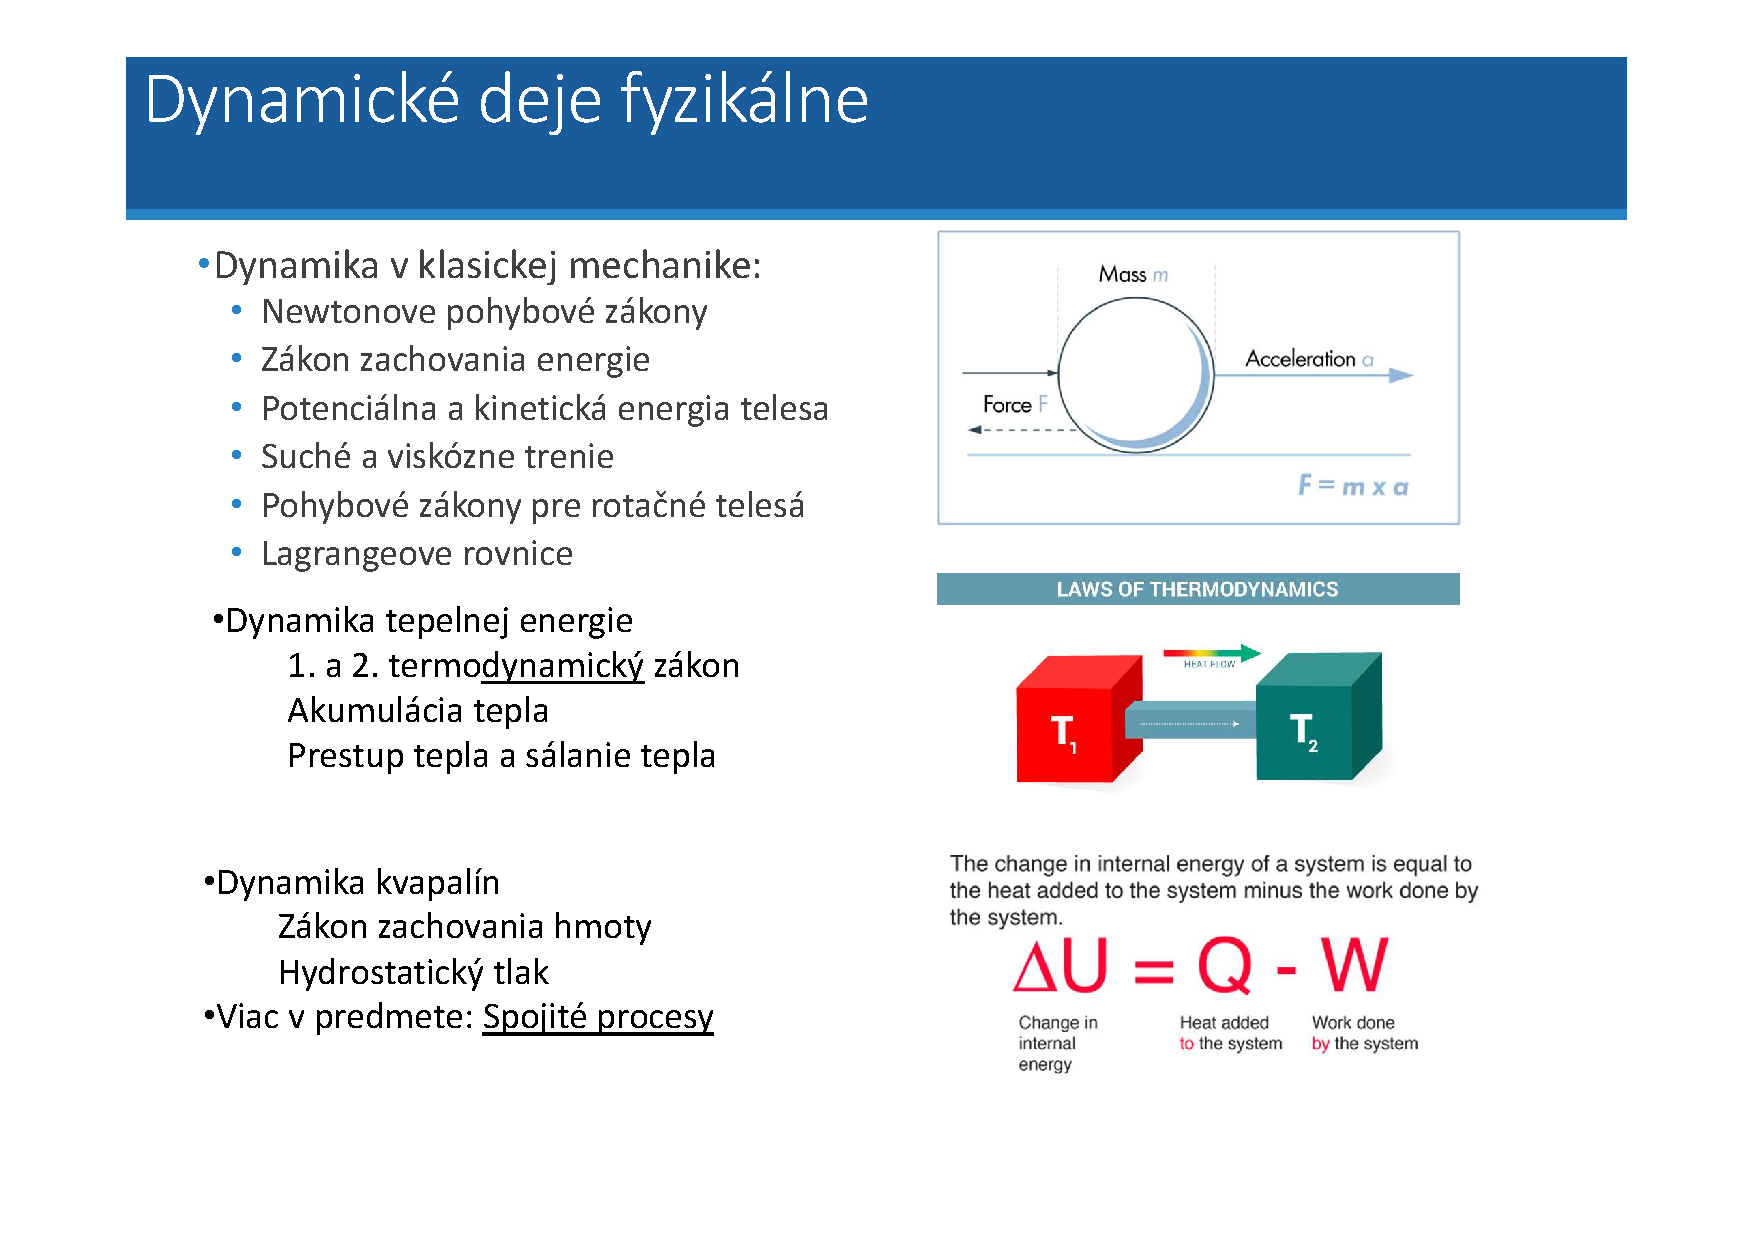
\includegraphics[width=1.36\textwidth]{P1_p19.pdf}}

    \vspace{-8mm}

    \makebox[\textwidth][c]{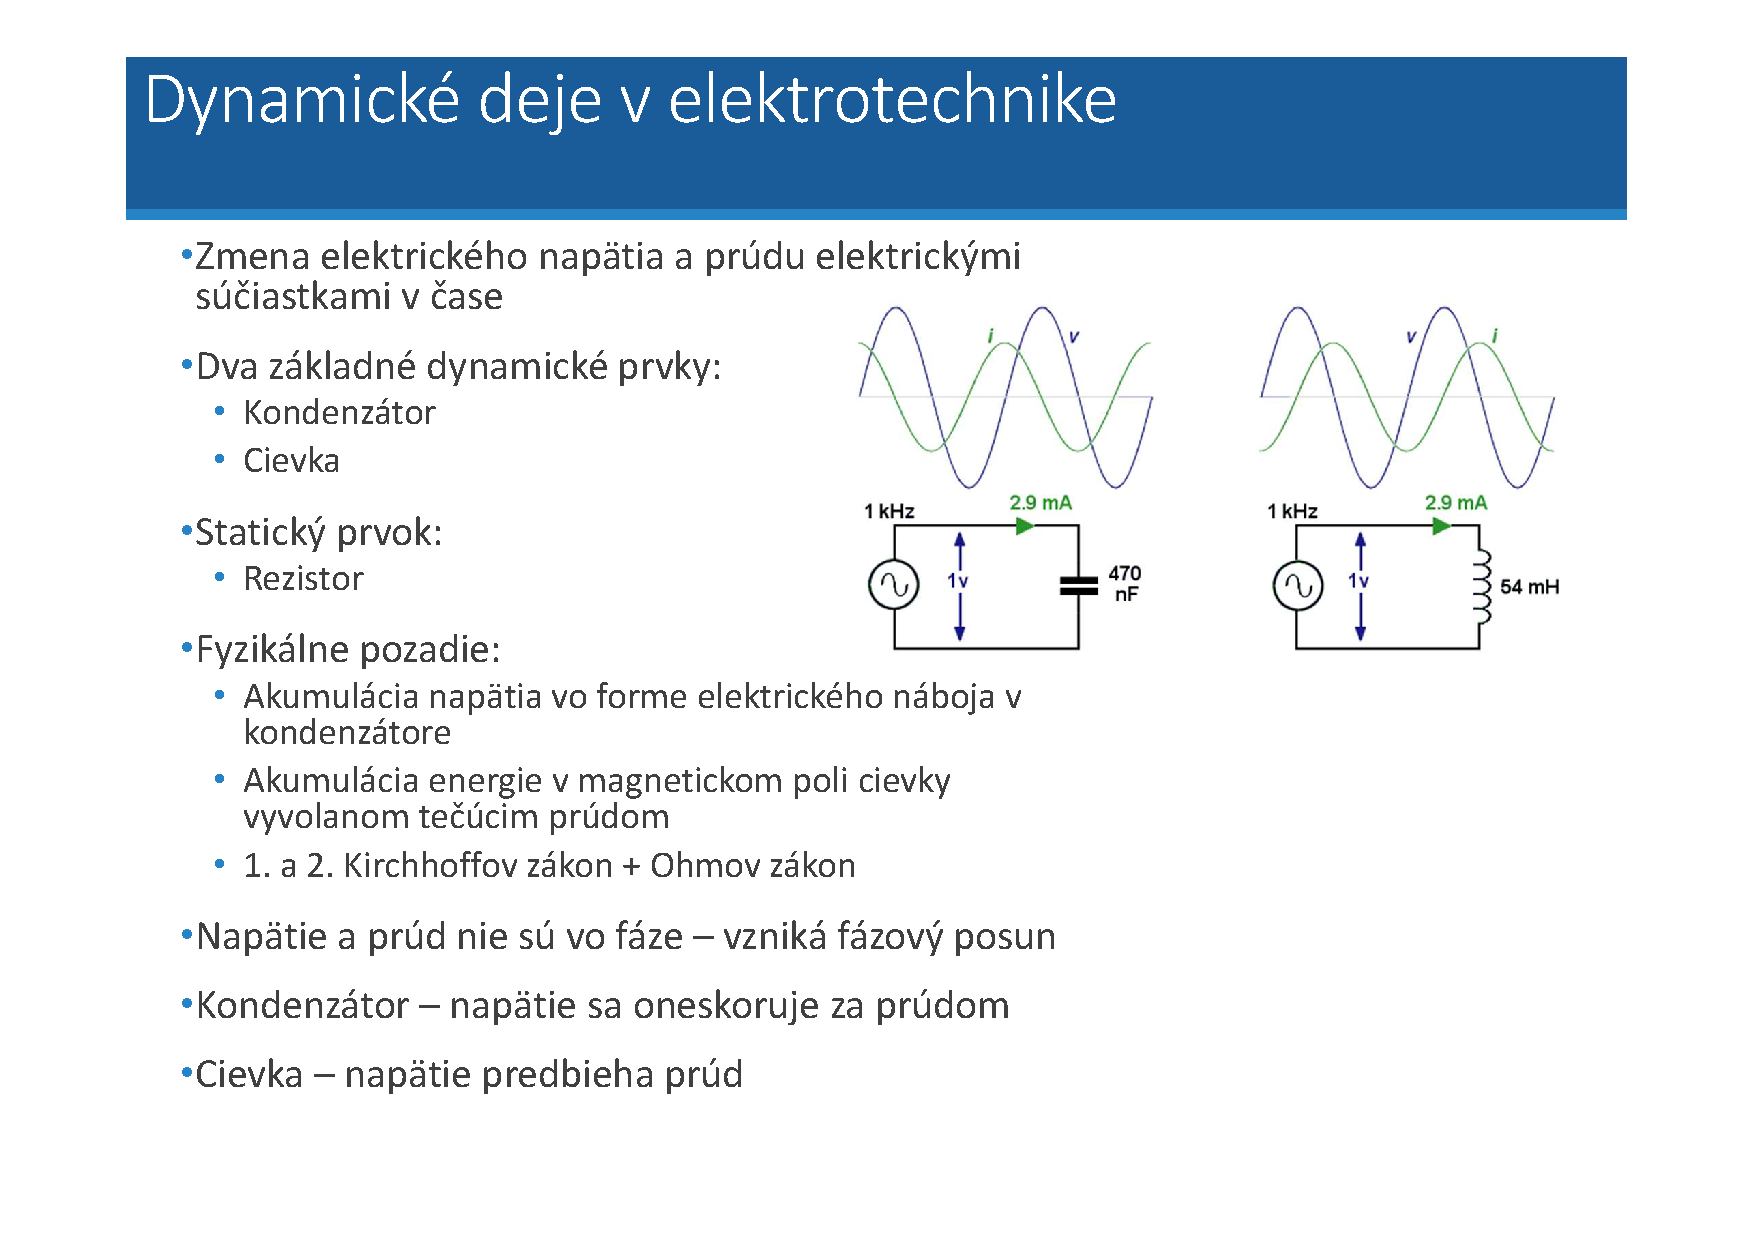
\includegraphics[width=1.36\textwidth]{P1_p20.pdf}}

\end{centering}

\pagebreak



\subsection{Riadenie procesov, riadenie systémov}

Jedným z najväčších prínosov kybernetiky je modelovanie a riadenie procesov.

Najskôr modelovanie „jednoduchých“ technických procesov:
\begin{itemize}
    \item Elektrické články a procesy
    \item Tepelné procesy
    \item Hydraulické procesy
    \item Mechanické procesy
    \item Chemické procesy
\end{itemize}

Teraz všetky druhy procesov od rakiet cez zložité technické procesy až po modely biologických procesov\ldots











\section{Konkrétne ilustračné príklady}



\subsection{Zosilnenie rezistorového deliča napätia}
\label{zrdn}


Uvažujme klasický odporový delič ako je znázornené na nasledujúcom obrázku.


\begin{figure}[!h]
	\centering

	\makebox[\textwidth][c]{%
	\input{../fig_standalone/OdporovyDelic.pdf_tex}
	}

	\caption{Odporový delič}
	\label{OdporovyDelic}
\end{figure}



Vstupom uvažovaného systému nech je napätie označené ako $u(t)$ a výstupným signálom nech je napätie $y(t)$.


\paragraph{Otázky}
\begin{itemize}[leftmargin=0pt, labelsep=4mm, itemsep=0pt]

	\item Nech hodnota vstupného signálu je konštantná, nemení sa, je ustálená. Aká je hodnota výstupného signálu, pričom pre jej určenie poznáme hodnoty rezistorov $R_1$ a $R_2$.

    \item Ako by ste definovali zosilnenie uvažovaného systému?

    \item Aká je veľkosť zosilnenia uvažovaného?

\end{itemize}



\subsection{Vybíjanie kondenzátora -- matematický model procesu}
\label{castVybij}

Majme RC obvod ako je znázornené na obr.~\ref{RCobvod}.

\begin{figure}[!t]
	\centering

	\makebox[\textwidth][c]{%
	\input{../fig_standalone/RCobvod.pdf_tex}
	}

	\caption{RC obvod}
	\label{RCobvod}
\end{figure}

Nech je na začiatku, v čase $t=0$, kondenzátor $C$ nabitý a na jeho svorkách je napätie s~hodnotou $u_0$. Inými slovami napätie $u(t)$ v čase $0$ je $u_0$, teda $u(0) = u_0$.

Ku kondenzátoru $C$ je pripojený rezistor $R$ a preto sa kondenzátor s rastúcim časom vybíja.


\paragraph{Diferenciálna rovnica}

Zostavme diferenciálnu rovnicu, ktorá opisuje proces vybíjania kondenzátora.


Pre kondenzátor platí
\begin{equation} \label{nabojDef}
    Q = CU
\end{equation}
čo znamená, že elektrický náboj $Q$ nazhromaždený v kondenzátore je úmerný napätiu na svorkách kondenzátora $U$ (azda priveľmi zjednodušene povedané, čitateľ si však iste vie dohľadať podrobnosti). Parameter $C$ predstavuje, ako je iste zrejmé, kapacitu kondenzátora.

Ak sa kondenzátor vybíja, mení sa náboj. Preto má zmysel vyšetrovať časový priebeh veľkosti náboja. Tým sa získa celkový prehľad aj o ďalších veličinách súvisiacich s procesom vybíjania kondenzátora.

Časová zmena elektrického náboja je elektrický prúd, teda
\begin{equation} \label{dQeqn}
    \frac{\text{d}Q}{\text{d}t} = - I
\end{equation}
kde $I$ je elektrický prúd a dôvodom záporného znamienka je, že smer elektrického prúdu sa značí práve opačne ako smer pohybu záporného náboja.

Rovnica \eqref{dQeqn} je v princípe diferenciálnou rovnicou. Obsahuje časovú deriváciu veličiny -- elektrického náboja. V tomto tvare však rovnicu nie je možné použiť na získanie časového priebehu samotnej veličiny (elektrického náboja). Totiž neznáme je nie len $Q$ ale v podstate aj $I$.



\bigskip

Namiesto veličiny $I$ by bolo vhodné mať na pravej strane rovnice \eqref{dQeqn} veličinu $Q$.
Z Ohmovho zákona plynie
\begin{equation} \label{ohmPrud}
    I = \frac{U}{R}
\end{equation}
Napätie $U$, ktoré sa týka nášho problému, je vo vzťahu k veličine $Q$, viď rovnicu  \eqref{nabojDef}. Konkrétne
\begin{equation} \label{nabojDef2}
    U = \frac{Q}{C}
\end{equation}
Dosadením \eqref{nabojDef2} do \eqref{ohmPrud} sa získa
\begin{equation} \label{ohmPrud2}
    I = \frac{Q}{RC}
\end{equation}
a následne dosadením \eqref{ohmPrud2} do \eqref{dQeqn}
\begin{equation} \label{diffRalpha}
    \frac{\text{d}Q}{\text{d}t} = - \frac{1}{RC} Q
\end{equation}

Diferenciána rovnica \eqref{diffRalpha} obsahuje jednu neznámu. Neznámou je veličina $Q$. Všeobecnejšie povedané, neznámou je časový priebeh veličiny. Neznámou je teda funkcia času. Preto píšme, že sa zaoberáme signálom (veličinou) $Q(t)$. Hodnoty $R$ a~$C$ sú len pevné hodnoty odporu a kapacity (viď obr.~\ref{RCobvod}). Neuvažujeme, že by sa menili v čase. Preto ich neoznačujeme ako signál (funkciu času). Teda signál označujme ako napr. $Q(t)$ a~konštantu ako napr. $R$.

Typicky, a pre zjednodušenie, sa rovnice \eqref{diffRalpha} zapisuje aj v tvare
\begin{equation} \label{diffR}
    \dot Q(t) = - \frac{1}{RC} Q(t)
\end{equation}
kde bodka $\dot{}$ označuje deriváciu podľa času rovnako ako operátor $\frac{\text{d}}{\text{d}t}$.


\bigskip

Riešením rovnice \eqref{diffR} je nejaká časová funkcia, nejaký signál, nejaký časový priebeh, konkrétne časový priebeh elektrického náboja, ktorý tu označujeme ako $Q(t)$.

Pre nájdenie jednoznačného riešenia je potrebné doplniť úlohu o začiatočnú podmienku. To je podmienka, ktorú musí spĺňať hľadaný signál $Q(t)$ na začiatku, teda v čase $t=0$. Pripomeňme, že napätie pred vybíjaním je dané (známe) a má hodnotu $u_0$. Je teda zrejmé, že je známa aj hodnota $Q(0) = C u_0$. Pre zjednodušenie označme ako $Q(0) = Q_0$.




\subsubsection{Náčrt riešenia diferenciálnej rovnice separáciou premenných}

Zaoberáme sa problémom v tvare
\begin{equation} \label{diffRbeta}
    \frac{\text{d}Q(t)}{\text{d}t} = - \frac{1}{RC} Q(t) \qquad Q(0) = Q_0
\end{equation}
kde $Q(t)$ je neznáma časová funkcia. Konštanty (nezávislé od času) $R$, $C$ a aj $Q_0$ sú známe. V rovnici je však ešte jedna premenná a tou je čas $t$. Ten, ako je známe, si len tak plynie. Je premennou pretože sa napríklad „podľa neho derivuje“.



\noindent
\hrulefill

\paragraph{Mimochodom}
\begin{itemize}
    \item Aké jednotky (rozmer) má výraz $RC$ v rovnici \eqref{diffRbeta}?
\end{itemize}
\noindent
\hrulefill

\medskip

Upravme diferenciálnu rovnicu \eqref{diffRbeta} tak, aby rovnaké premenné boli na rovnakých stranách. V tvare \eqref{diffRbeta} je signál $Q(t)$ na oboch stranách rovnice. Nech je len na ľavej strane. Rovnako, nech čas $t$ je len na pravej strane. Teda
\begin{equation} \label{diffRbeta2}
    \frac{1}{Q(t)}\text{d}Q(t) = - \frac{1}{RC} \text{d}t
\end{equation}

Všimnime si, že teraz je možné obe strany rovnice integrovať, každú podľa vlastnej premennej, teda
\begin{equation} \label{diffRbeta3}
    \int \frac{1}{Q(t)}\text{d}Q(t) =  \int - \frac{1}{RC} \text{d}t
\end{equation}
Výsedkom inegrovania je
\begin{equation} \label{diffRbeta4}
     \ln \left(  Q(t)  \right) + k_1 =   - \frac{1}{RC} t + k_2
\end{equation}
kde $k_1$ a $k_2$ sú konštanty vyplývajúce z neurčitých integrálov (a tiež sme potichu uvážili, že $Q(t)$ nebude nadobúdať záporné hodnoty).





\bigskip

Rovnica \eqref{diffRbeta4} už nie je diferenciálna. Žiadna veličina v nej nie je derivovaná podľa času.

Vyjadrime z rovnice \eqref{diffRbeta4} signál $Q(t)$. Úpravou
\begin{align}
    \ln \left(  Q(t)  \right)  =   - \frac{1}{RC} t + k_3
\end{align}
sme zaviedli konštantu $k_3 = k_2 - k_1$. Ďalej
\begin{subequations}
    \begin{align}
        Q(t)   &=  e^{\left( - \frac{1}{RC} t + k_3 \right)} \\
        Q(t)   &=  e^{\left( - \frac{1}{RC} t \right)}  e^{k_3} \label{rawRies}
    \end{align}
\end{subequations}

Už v tomto bode je rovnica \eqref{rawRies} predpisom, ktorý udáva časovú závislosť veličiny $Q$. Vyjadruje signál (časovú funkciu) $Q(t)$. Časová funkcia $Q(t)$ je riešením diferenciálnej rovnice \eqref{diffRbeta2}.

V rovnici \eqref{rawRies} je konštanta $e^{k_3}$. Je to všeobecná konštanta a môže mať akúkoľvek hodnotu. Je možné ukázať, my si tu však dovolíme neuviesť formálnu ukážku, že táto konštanta je daná začiatočnou podmienkou priradenou k diferenciálnej rovnici. V~tomto prípade platí $e^{k_3} = Q_0$.

Hľadaným riešením diferenciálnej rovnice je časová funkcia v tvare
\begin{align}
    Q(t)   &=  Q_0 \ e^{\left( - \frac{1}{RC} t \right)}   \label{rawRies2}
\end{align}


\noindent
Funkcia je graficky znázornená na obrázku~\ref{Graffunkcie}.











\begin{figure}[!t]
	\centering

	\makebox[\textwidth][c]{%
	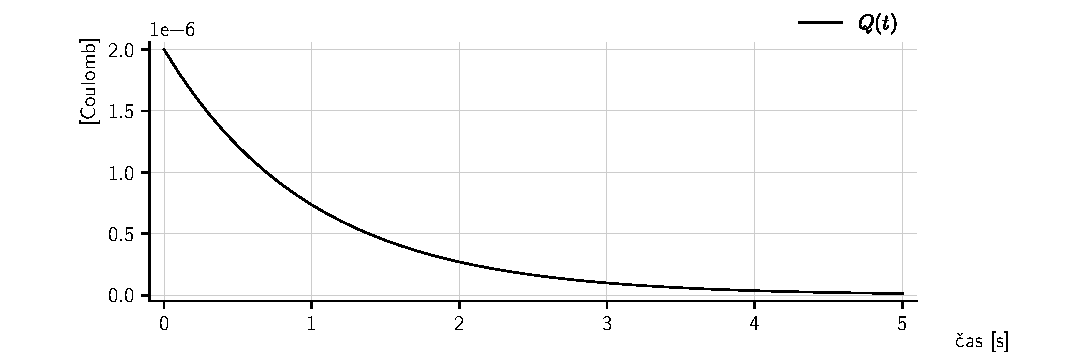
\includegraphics{../fig/cv01_fig_1.pdf}
	}

	\caption{Graf funkcie \eqref{rawRies2} pre $R = 10^6$ [$\Omega$], $C = 1$ [$\mu$F] a $Q_0 = 2\cdot 10^{-6}$ [Coulomb] (ľubovolné hodnoty len ako príklad)}
	\label{Graffunkcie}
\end{figure}



\begin{figure}[!b]
	\centering

	\makebox[\textwidth][c]{%
	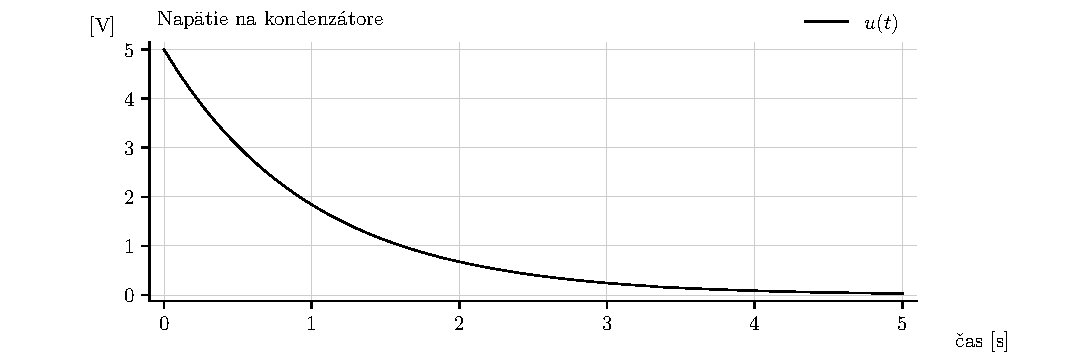
\includegraphics{../fig/cv01_fig_2.pdf}
	}

	\caption{Časový priebeh napätia na kondenzátore}
	\label{PriebehNapatieDefault}
\end{figure}







\subsubsection{Časový priebeh napätia na kondenzátore}


Vyšetrili sme časový priebeh elektrického náboja počas vybíjania kondenzátora. Opis situácie na začiatku časti~\ref{castVybij} však nepriamo predpokladá, že sa budeme venovať napätiu. Vzájomný vzťah už poznáme, a jeho formálne presnejší zápis (napätie $u(t)$ ako signál) je
\begin{equation} \label{QUsig}
    u(t) = \frac{1}{C} Q(t)
\end{equation}
Takže ak poznáme priebeh $Q(t)$, poznáme aj priebeh $u(t)$.

Začiatočnú podmienku pre signál $Q(t)$, teda hodnotu $Q(0)$ samozrejme tiež možno určiť so želanej (danej) začiatočnej podmienky signálu $u(t)$.
\begin{equation}
    Q(0) = C u_0
\end{equation}





\bigskip

\noindent
V zmysle úvodu časti~\ref{castVybij} uvažujme nasledujúci príklad
\begin{align*}
    C &= 1 \text{ [$\mu$F]} \\
    R &= 10^6  \text{ [$\Omega$]} \\
    u_0 &= 5  \text{ [V]}
\end{align*}
Pre tento príklad je následne začiatočná podmienka pre signál $Q(t)$
\begin{equation}
    Q(0) = 10^{-6} \cdot 5 = 0.000050 \text{ [Coulomb]}
\end{equation}
Výsledný priebeh napätia je zobrazený na obr.~\ref{PriebehNapatieDefault}.









\subsubsection{Príklady pre rôzne parametre $R$ a $C$}


Pre zaujímavosť, ukážme priebeh napätia pre rôzne parametre $R$ a $C$. Príklady sú sumarizované v tabuľke~\ref{Príklady rôznych parametrov}. Graficky znázornené časové priebehy na obr.~\ref{PriebehNapatiePriklady}.



\begin{figure}[!t]
	\centering

    \vspace{-3mm}

	\makebox[\textwidth][c]{%
	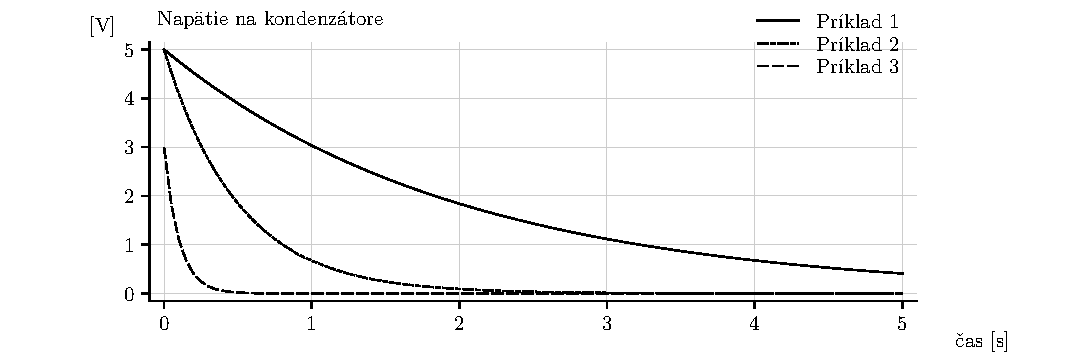
\includegraphics{../fig/cv01_fig_3.pdf}
	}

    \vspace{-3mm}

	\caption{Časový priebeh napätia na kondenzátore}
	\label{PriebehNapatiePriklady}

    \vspace{-3mm}

\end{figure}



\begin{table}[!t]
	\centering

	\caption{Príklady rôznych parametrov}
	\label{Príklady rôznych parametrov}

	\begin{tabular*}{\textwidth}{  l @{\extracolsep{\fill}} ccc }
		\toprule
            & $C$ [F] & $R$ [$\Omega$] & $u_0$ [V] \\
        \midrule
		Príklad 1 & $ 2 \cdot 10^{-6}$  & $10^{6}$  & 5 \\
		\midrule
		Príklad 2 & $\frac{1}{2} \cdot 10^{-6}$ & $10^{6}$  & 5 \\
		\midrule
		Príklad 3 &  $10^{-6}$ &  $ \frac{1}{10} \cdot 10^{6}$ & 3 \\
		\bottomrule
	\end{tabular*}
\end{table}









\subsection{Príklad využitia výpočtového softvéru pre časť~\ref{castVybij}}




Na obrázku~\ref{Graffunkcie} je znázornená funkcia \eqref{rawRies2}. Ak by sme chceli túto funkciu graficky znázorniť s využitím jazyka Python (avšak v princípe akéhokoľvek skriptovacieho jazyka), v rámci ktorého využijeme knižnice \lstinline|NumPy| a \lstinline|Matplotlib|, mohlo by to vyzerať nasledovne:

% {\catcode`\-=12
\begin{lstlisting}[
    language=Python,
    % caption={Pre viac pozri \lstinline|PY/MRS01_section_02.ipynb|},
    ]
timeVect = np.arange(0,5.1,0.1)

R = 10**6
C = 10**-6
Q_0 = 2*10**-6

riesFcia = Q_0 * np.exp( (-1.0/(R*C)) * timeVect )

plt.plot(timeVect, riesFcia)
\end{lstlisting}
% \lstinputlisting[language=Python,
%                  caption={Súbor \lstinline{MRS01_kTextu.py}},
%                  % label={vypk01},
% 				 consecutivenumbers=false,
% 				 % linerange={34-42}
% 				 linerange=c01-c01,
%                  ]{../../PY/MRS01_kTextu.py}
% }

\noindent
Viac je táto téma rozvinutá v \lstinline|jupyter| notebooku \lstinline|PY/MRS01_section_02.ipynb|.


\bigskip

\noindent
\hrule

\medskip

\noindent
Ak sa tu čitateľ prvý krát stretáva s Python-om pre numerické výpočty, azda užitočnými mu budú tieto odkazy:

\paragraph{Python (inštalovaný ako distribúcia balíčkov...)}
Pre všeobecné používanie Python-u na Windows, obzvlášť pre „vedecké výpočty“, sa čitateľovi odporúča, tak ako sa uvádza aj tu: \url{https://www.scipy.org/install.html}, distribúcia Anaconda: \url{https://www.anaconda.com/}


\medskip

\noindent
Ak nie je výslovne uvedené inak, používa sa tu Python vo verzii 3.

\paragraph{Jupyter}
V týchto súvislostiach je vhodné tiež upozorniť na \url{https://jupyter.org/}. IPython ako aj Jupyter notebook sú súčasťou distribúcie Anaconda.

\paragraph{Spyder}
Možno pre úplnosť, Spyder (\url{https://github.com/spyder-ide}) je IDE obsiahnuté v~distribúcii Anaconda, ktoré je zamerané na takpovediac vedecké účely (skriptovanie, práca s dátami atď. - nie „programovanie“ vo všeobecnosti).

\medskip

\noindent
\hrule

% \bigskip




% Samotná časová funkcia \eqref{rawRies2} je analytickým riešením diferenciálnej rovnice \eqref{diffR}. Ako však bez znalosti tohto analytického riešenia získať obrázok~\ref{Graffunkcie} (teda vyriešiť diferenciálnu rovnicu)?

% Len ako prvý kontakt tu uveďme istý spôsob získania tzv. \emph{numerického riešenia diferenciálnej rovnice}. Tejto a súvisiacim témam sa budeme podrobne venovať v~ďalších textoch, tu nech je to len takpovediac prvá ukážka.

% V prvom rade vytvorme funkciu, ktorá bude realizovať to čo „robí“ (bez ďalšieho písomného vysvetlenia v tomto texte) diferenciálna rovnica, teda:

% {\catcode`\-=12
% \lstinputlisting[language=Python,
%                  caption={Súbor \lstinline{MRS01_kTextu.py}},
% 				 consecutivenumbers=false,
% 				 linerange=c02-c02,
%                  ]{../../PY/MRS01_kTextu.py}
% }

% Túto funkciu využije istý nástroj, ktorý je schopný zostaviť numerické riešenie - tu konkrétne nájde y-súradnice k požadovaným x-súradniciam. X-súradnice sú v tomto prípade čas (na x-osi je čas). Uvedený nástroj sa nazýva \emph{ODE solver} -- „riešič“ obyčajných diferenciálnych rovníc. Zrealizujme nasledovné:

% {\catcode`\-=12
% \lstinputlisting[language=Python,
%                  caption={Súbor \lstinline{MRS01_kTextu.py}},
% 				 consecutivenumbers=false,
% 				 linerange=c03-c03,
%                  ]{../../PY/MRS01_kTextu.py}
% }

% Máme teda funkciu, ktorej „povieme“ \lstinline|t_start, t_final, T_s|, teda časové hodnoty od-do kedy chcem mať numerické riešenie a s akým časovým krokom. Ďalej v nej vieme zadávať (meniť) parametre \lstinline|param|, čo, ako vidíme, sú v tomto prípade parametre systému, ktorým sa tu zaoberáme (elektrický odpor $R$ a kapacita $C$). ODE solver sa tu nazýva \lstinline|odeint|.

% Túto funkciu sme nazvali, že „simulácia“, pretože v istom zmysle ide o simuláciu dynamického systému. Nastavme teda túto pomyselnú simuláciu:

% {\catcode`\-=12
% \lstinputlisting[language=Python,
%                  caption={Súbor \lstinline{MRS01_kTextu.py}},
% 				 consecutivenumbers=false,
% 				 linerange=c04-c04,
%                  ]{../../PY/MRS01_kTextu.py}
% }

% Zavolaním našej funkcie tú simuláciu vykonajme:

% {\catcode`\-=12
% \lstinputlisting[language=Python,
%                  caption={Súbor \lstinline{MRS01_kTextu.py}},
% 				 consecutivenumbers=false,
% 				 linerange=c05-c05,
%                  ]{../../PY/MRS01_kTextu.py}
% }

% Týmto sme ukázali príklad využitia výpočtového softvéru v téme, ktorej sa venuje tento text.














\section{Cvičenie prvé}


\subsection{Úlohy}

\begin{enumerate}[leftmargin=0pt, labelsep=4mm, itemsep=0pt]

    % \color{Red}

    \item Odpovedajte na otázky uvedené v časti~\ref{zrdn}.

	\item Zostavte diferenciálnu rovnicu, ktorá opisuje proces vybíjania kondenzátora.

    \item Určte jednotky (rozmer) všetkých parametrov a signálov (veličín) v zostavenej rovnici.

    \item Nájdite analytické riešenie uvedenej diferenciálnej rovnice.

    \item Nakreslite graf časovej funkcie, ktorá je analytickým riešením diferenciálnej rovnice. Potrebné číselné hodnoty parametrov a signálov nech sú ľubovolné.

    \item Nájdite numerické riešenie diferenciálnej rovnice (s využitím Simulinku).

\end{enumerate}

\subsection{Poznámky}


\paragraph{Simulink (MATLAB)}

Zaoberáme sa problémom v tvare
\begin{equation} \label{diffRbeta222}
    \frac{\text{d}Q(t)}{\text{d}t} = - \frac{1}{RC} Q(t) \qquad Q(0) = Q_0
\end{equation}
kde $Q(t)$ je neznáma časová funkcia. Konštanty (nezávislé od času) $R$, $C$ a aj $Q_0$ sú známe.


\begin{center}

    \vspace{-1mm}

    \makebox[\textwidth][c]{%
	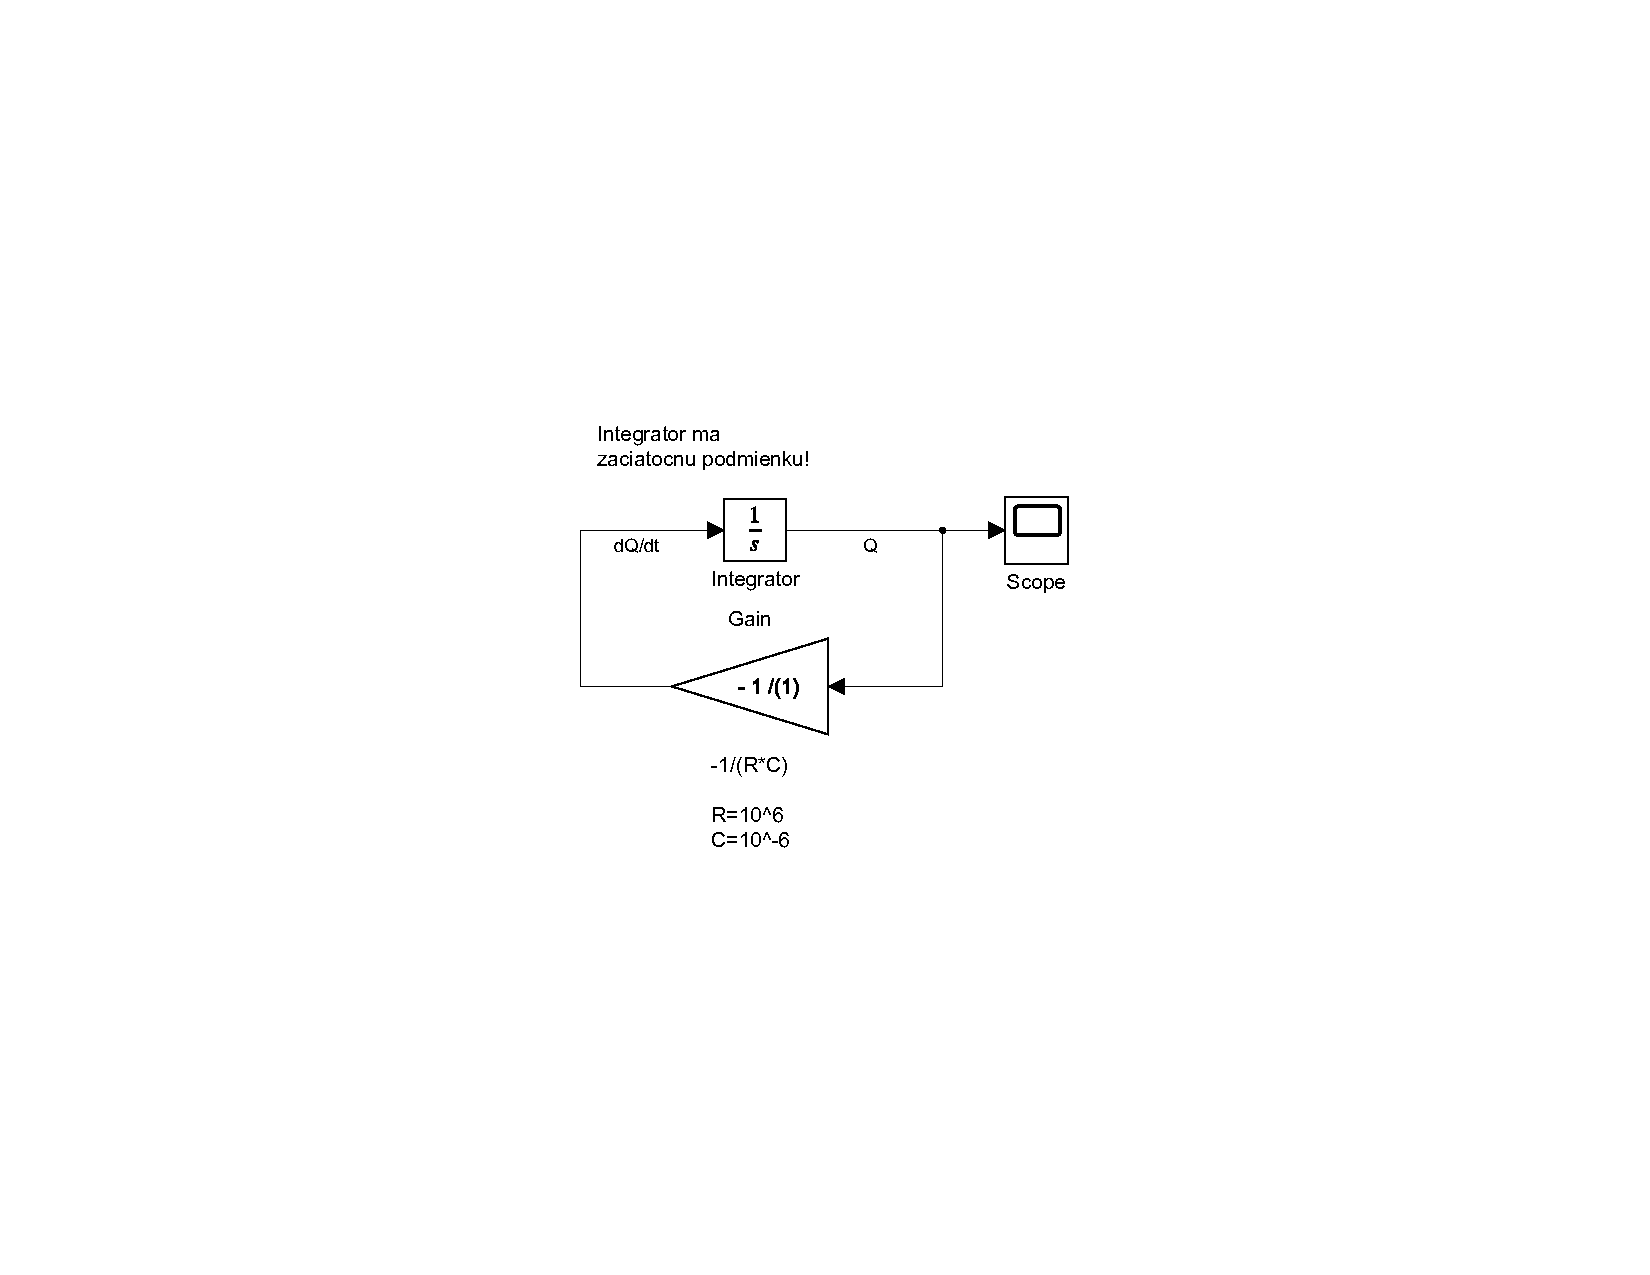
\includegraphics[trim=65mm 65mm 65mm 65mm, clip, scale=0.75]{sim_Q.pdf}
	}

    \vspace{-5mm}

	\figcaption{Simulačná schéma zodpovedajúca rovnici  \eqref{diffRbeta222}}
	\label{sim_Q}

    \vspace{-1mm}

\end{center}




\paragraph{ODE solver (MATLAB)}

Pre numerický výpočet riešenia pomocou procedúry \verb|ode45| je potrebné predmetný systém (rovnicu) zapísať ako funkciu, ktorú bude procedúra \verb|ode45| používať. V tomto prípade:
\begin{lstlisting}[language=Matlab,]
function dQ = fundif(t,x);
R = 10^6;
C = 10^(-6);
Q = x;
dQ = -(1/(R*C)) * Q;
\end{lstlisting}
Je potrebné vytvoriť samostatný súbor \verb|fundif.m|, ktorý bude obsahovať uvedenú fuknciu, tak ako je tu uvedené.

Mimochodom, na tomto mieste nebudeme (tu v texte) uvádzať podrobnosti k~ODE solveru. Cieľom je tu len oboznámiť čitateľa s možnosťami ako získať numerické riešenie. Ako to „funguje“ bude jemne komentované neskôr.

Samotné použitie procedúry \verb|ode45| sa vykoná nasledovnými príkazmi (povedzme v skripte v inom m-súbore):
\begin{lstlisting}[language=Matlab,]
Q_0 = 2 * 10^(-6);
[t,y] = ode45('fundif',[0 5],[Q_0]);
plot(t,y)
\end{lstlisting}
Obrázok sa ponecháva na čitateľa\ldots











\section{Otázky a úlohy}

\begin{enumerate}[leftmargin=0pt, labelsep=3mm, itemsep=0pt]

	\item Vysvetlite pojem \emph{zosilnenie systému} (alebo \emph{statické zosilnenie systému}).

    \item Ako sa nazýva pomer medzi ustálenou hodnotou výstupného signálu systému a~ustálenou hodnotou vstupného signálu systému? 
    	
    \item Vysvetlite rozdiel medzi statickým a dynamickým systémom.

    {\color{Gray} \scriptsize Statickým nazývame taký systém, pri ktorom je vhodné (či užitočné) zanedbať zotrvačnosť (mechanickú, tepelnú a~podobne). Výstupná veličina statického systému sa mení okamžite, bez vplyvu zotrvačnosti.}
    
    \item Čo sú to \emph{začiatočné podmienky} dynamického systému?
    
    \item Vlastnými slovami vysvetlite pojem \emph{Kybernetika} (čo je to Kybernetika).

\end{enumerate}



\renewcommand{\refname}{Odporúčaná literatúra}

\nocite{AsM08se}
\bibliography{../misc_LaTeX/Bib_MRS}{}
\bibliographystyle{plain}






\end{document}
